\chapter{Rizika nanotechnologií}

Hodnocení rizik nanotechnologií vychází z tradičního pojetí hodnocení rizik makromateriálů. Hodnocení bezpečnosti látek je složeno ze tří částí - hodnocení rizika, řízení rizika a komunikaci o riziku. Samotné hodnocení rizika je složeno ze čtyř kroků, jak je zobrazeno na obrázku \ref{fig:hodnoceni_rizik}. Prvním krokem je identifikace nebezpečí dále jeho popis, hodnocení expozice a odhad rizika. Řízení rizika je zaměřeno na tvorbu legislativních opatření a jejich praktické zavádění. Následně státní dozor dohlíží na dodržování těchto předpisů. Poslední komunikace o riziku je důležitou součástí především pro sdílení informací a výsledků hodnocení rizik. \cite{filipova2012} \\



\begin{figure}
    \centering
    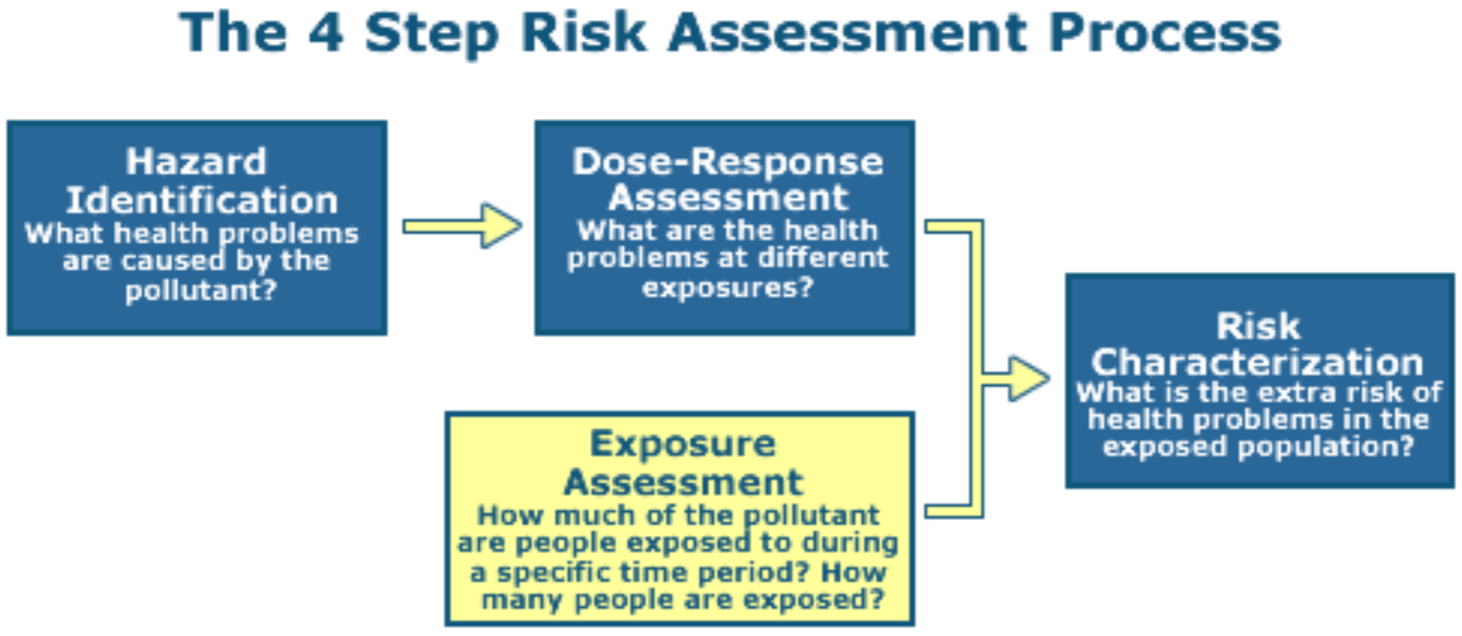
\includegraphics[width=0.75\textwidth]{pictures/hodnoceni_rizika.png}
    \caption{Schéma identifikace rizik. \cite{filipova2012}}
    \label{fig:hodnoceni_rizik}
\end{figure}
    
\section{Cesty vstupu do organismu}

Nejvýznamější cestou vstupu nanočástic do organismu je inhalace. Částice větší než deset mikrometrů se zachytí ve sliznici na skořepě nosní. Menší částice prochází až do průdušek a plicních sklípků. Nanočástice mohou být buď hlenovým eskalátorem vyplavovány z plic nebo podléhají fagocytóze alveolárních makrofágů. \cite{nohavica2011}  Mohou se také navázat na různé proteiny a s nimi se dostat do krevního řečiště a lymfatického systému. Dalším možným vstupem je čichový nerv, který umožňuje nanočásticím přímý vstup do mozku. \cite{filipova2012}\\

Příjem nanočástic perorální cestou je asi druhý nejrozšířenější. Mechanismy vstupu nejsou jednoznačné. Předpokládá se, že velká část příjmu probíhá stěnou střeva. Při těchto přechodech hraje roli nejen velikost nanočástic - menší nanočástice snadněji prostupují střevní stěnou - ale také povrchový náboj, který může zásadním způsobem ovlivňovat průchodnost epiteliem střev. \cite{filipova2012}\\

Vstup nanočástic neporušenou pokožkou představuje nízké riziko. Výzkumy ukazují, že i při jiných cestách vstupu je důležitý vstup přímo přes buňky a nikoliv mezibuněčnými prostory. Pokožka tvořená zrohovatělými buňkami tedy představuje účinnou bariéru pro vstup nanočástic. Vyšší prostupnost pokožkou mají lypofilní nanočástice, které prostupují chlupy nebo potními žlázami. Hydrofóbní a iontové nanočástice kožní bariéru překonávají obtížně. \cite{filipova2012} \\

Nanočástice představují větší riziko než klasické materiály z důvodu jejich snadného prostupu přes tělní bariéry. Klasické materiály většinou nemohou samostatně migrovat v organismu a po jejich rozpoznání dochází k jejich degradaci a vyloučení. Naopak nanočástice mohou migrovat kůží, dostávat se do tělních tekutin a dokáží překonat hematoencefalickou bariéru, čímž se dostávají přímo do mozku. Přechod placentární bariérou mezi matkou a plodem není dostatečně prozkoumán. Zvýšený povrch nanočástic zvyšuje jejich reaktivitu, která z hlediska hodnocení rizik může způsobovat interakci nanočástic s biomolekulami v buňkách. Nanočástice se mohou akumulovat v některém z orgánů a nemusí docházet k jejich vylučování, mohou interkalovat s molekulami RNA či DNA nebo mohou ovlivňovat metabolické dráhy.\\

\section{Rizika pro životní prostředí}

Nanomateriály jsou potenciálním rizikem pro životní prostředí. Jejich použití v lidské činnosti přináší zodpovědnost za jejich řízené šíření do životního prostředí. Stejně jako v lidském organismu se mohou akumulovat v tělech živočichů či rostlin a být tak zdrojem pro vstup do lidského těla. Některé nanomateriály mohou být toxické pro některé vyšší organismy. Toxicita vůči bakteriím a nižším organismům je často studovaná jako první krok ke stanovení toxicity nanomateriálů pro člověka. Mnoho nanočástic je antibakteriálních a využívají se k dezinfekci. \\

Zvýšené katalytické účinky některých nanočástic lze využít k čištění odpadních vod, rychlejší degradaci toxických či karcinogenních látek, ale tyto nanočástice je třeba poté z vod účinně odstranit. Je třeba sledovat přirozený koloběh nanočástic v biosféře. Současně je důležité si uvědomit, že nanočástice jsou přirozenou součástí biosféry. 


\section{Faktory ovlivňující toxicitu}

Při identifikaci rizik je třeba postupovat systematicky. Existuje mnoho faktorů, které ovlivňují toxicitu nanočástic. V první řadě je to chemické složení, jaké látky se mohou uvolňovat z povrchu nanočástic, velikost povrchu a inertnost nanočástic, která může způsobovat jejich snadnější prostupnost buněčnými membránami. Dále velikost nanočástic, obecně platí, že větší nanočástice jsou méně rizikové, ale je třeba rozlišovat velikost nanočástic a agregátů, které jsou sice velké, ale zachovávají povrch původního počtu nanočástic. Velikost nanočástic ovlivňuje schopnost selektivní kumulace uvnitř buněk. Zásadní vliv má také morfologie nanočástic = jejich tvar. Chemicky totožné nanočástice o stejné velikosti, ale různého tvaru mohou mít zcela odlišnou toxicitu. Dalšími charakteristickými vlastnostmi je rozpustnost nanočástic, povrchový náboj či adsorbované biomolekuly, lipofilita, biodegrabilita a persistence. Pro plné zhodnocení rizik je nutné charakterizovat nanočástice ve všech formách, ve kterých se vyskytují -  ihned po výrobě, v produktech, v matrici, ve formě, ve které jsou přítomny v biologických tkáních a tělních tekutinách. \\

Z hlediska toxicity a hodnocení rizik je dalším důležitým parametrem doba expozice působení nanočástic a dávka, které je organismus vystaven. Charakterizaci rizik je třeba doplnit o testy toxicity, pomocí nichž lze plně charakterizovat rizika, jak ukazuje obrázek \ref{fig:hodnoceni_rizika}.

    \begin{figure}[h]
        \centering
        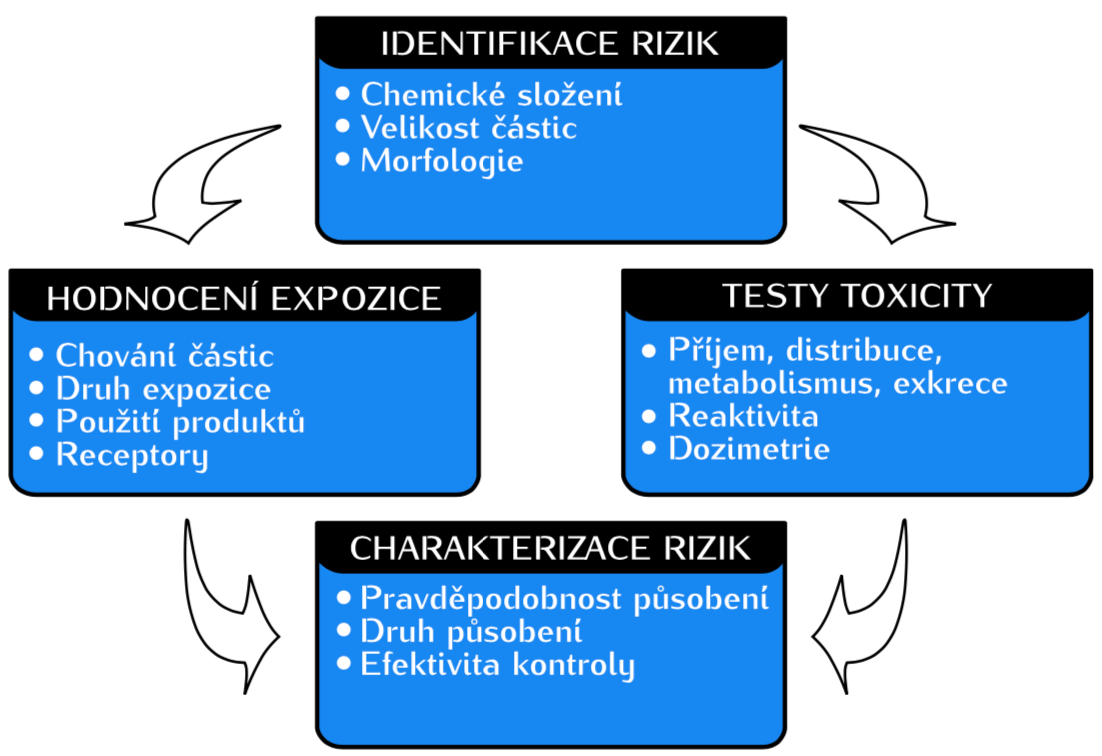
\includegraphics[width=0.75\textwidth]{pictures/hodnoceni_rizik.png}
        \caption{Hodnocení rizik nanotechnologií. \cite{filipova2012}}
        \label{fig:hodnoceni_rizika}
    \end{figure}

\section{Indikátory potenciálního rizika nanomateriálů}

Evropský úřad pro bezpečnost potravin (EFSA) v roce 2011 vydal doporučení pro odhadování rizik nanomateriálů. \cite{filipova2012} V roce 2018 EFSA vydala aktualizaci těchto doporučení, viz \cite{efsa2018}.\\

\noindent \textbf{Indikátory potenciální toxicity}
    \begin{itemize}
        \item vysoká míra reaktivity (př. katalytická, chemická, biologická),
        \item komplexní morfologie/rigidní, dlouhé trubky nebo vlákna, vysoký poměr šířky k délce nanomateriálů, fullereny, krystalová struktura, porozita, multifunkční nanomateriály,
        \item interakce s biomolekulami jako enzymy, DNA, receptory, efekt Trojského koně,
        \item celková transformace (např. stáří, změny povrchových vlastností, porozita) nebo metabolity (př. změny nebo ztráty obalení – dynamická korona),
        \item nanočástice zamýšlené pro využití jako antibakteriální prostředky\\
    \end{itemize}
    
\noindent \textbf{Potenciální indikátory pro vysokou expozici}
    \begin{itemize}
        \item vysoký produkční objem na poli aplikací,
        \item vysoká mobilita nanoformy v organismu (pravděpodobná interní expozice) (př. transport skrz makrofágy, transport skrz buněčné membrány, přes bariéru krev–mozek, anebo bariéru placenty (nosiče léčebných látek) a mobilizační potenciál (př. infiltrace, sorpce, vytváření komplexů),
        \item cílené nebo kontrolované uvolňování,
        \item persistence/stabilita (př. ve vodě, v tucích, tělních tekutinách, nedostatek rozpustnosti nebo degrability),
        \item bioakumulace.\\
    \end{itemize}
    
\noindent \textbf{Indikátory možné ztráty nanovlastností - možnost hodnocení konvenčním hodnocením rizik}
    \begin{itemize}
        \item vzrůstající míra rozpouštění (ve vodě, potravinové matrici nebo v tělních tekutinách),
        \item rostoucí míra degradability (př. biologické nebo fotokatalytické) vzhledem k non-nanoformní degradaci produktů,
        \item přítomnost silně vázaných agregátů (př. určeno podmínkami produkce), fixovanými a permanentně vázanými v matricích (př. stabilita matrice, typ vazeb, chování před rozkladem).
    \end{itemize}